\documentclass[12pt]{article}
\usepackage{parskip}
\usepackage[letterpaper, margin=1in]{geometry}
\usepackage{graphicx}
\usepackage{amsmath}
\usepackage{pdflscape}
\usepackage{subcaption}
\usepackage{tikz}
\usepackage{enumitem}
\title{ELECENG 2EI5 Project 1}
\author{Raeed Hassan \\ hassam41 \\  \\ McMaster University}
\usepackage{fancyhdr}
\renewcommand{\headrulewidth}{0pt}
\usepackage{titlesec}
\fancypagestyle{lscapedplain}{%
  \fancyhf{}
  \fancyfoot{%
    \tikz[remember picture,overlay]
      \node[outer sep=1cm,above,rotate=90] at (current page.east) {\thepage};}
}
\begin{document}
\maketitle
\pagebreak
\section{Hand Design}
\begin{enumerate}[label=\alph*.]
    \item %Why did you choose a specific circuit topology? (So you need to show that you are aware of different topologies that can be used to achieve the required result, then explain why you chose the one that you did.)
    A DC power supply that converts an AC source into a DC power source consists of a transformer, a rectifier, a filter, and a regulator. We will determine the design and specifications of the first three components to meet the desired specifications of the project.
    
    The first two component of the that we will consider are the rectifier and the filter. Both half-wave and full-wave rectifiers can produce a DC output from an AC input with the appropriate filter. A RC parallel shunt filter was the filter of choice. Other possible filters such as choke filters and LC filters were investigated, however the RC parallel shunt filter performed the best in simulation.

    The two full-wave rectifier designs considered were the bridge rectifier and the centre-tapped rectifier. These are both full-wave rectifiers that should output an appropriate AC output. Both implementations of a full-wave rectifier would serve our purpose, so a decision was made on which circuit was easier to build with the hardware available to us. A bridge rectifier requires four diodes, and four identical diodes were not available to us. Using different diodes would only increase the complexity of our calculations, therefore the centre-tapped rectifier was the more practical full-wave rectifier design as we had two identical diodes that could be used to construct the circuit.

    The decision between using a centre-tapped rectifier and a half-wave rectifier ultimately came down to the hardware we had available for the construction of the circuit. Neither the desired resistor nor the desired capacitor were available for either circuit, however the capacitors available to us would put us closer to our desired value for centre-tapped rectifier than the half-wave rectifier.

    The centre-tapped rectifier was our circuit of choice. This meant that the design of the transformer was also fixed. The transformer had to be a centre-tapped transformer, that had two inverted outputs that would serve as the inputs to our circuit. In the construction of the circuit, we will use two two inverted waveforms from the wave generator to emulate the output of the transformer.

    The complete design of the circuit can be seen in Figure 1.

    \item %How did you calculate the component values needed for your circuit?
    The AC power source has a frequency of 1kHz and a voltage of 169.7V ($120V\cdot\sqrt{2}$). The resistor must be 300$\Omega$ as the output voltage and current are specified. $R = 300\Omega = \frac{3V}{10mA}$. The value of the capacitor is dependent on the voltage ripple. In a full-wave rectifier circuit, the voltage ripple with a shunt filter is equal to $V_r = \frac{I}{C\cdot2f}$. We can isolate for C to determine the capacitance of our desired filter. $C = \frac{I}{V_r \cdot 2f} = \frac{10mA}{0.1V \cdot 2 \cdot 1kHz} = 25\mu F$. The turn ratio (specifically the inductance ratio in the simulation) was determined using trial and error in simulation. The circuit outputs met the desired specifications when the input of the rectifier circuit was 3.86V. This corresponds to a turn ratio of approximately $\frac{44}{1}$.

    \item %What design tradeoffs, design margins, component ratings, safety, and other issues did you take into account in your design? (This point is very important – you must show that you considered safety issues and component ratings in your design and you must show that you have an understanding of design margins and tradeoffs.)
    All potential components of the recitifier/filter circuit could be substituted with various available components, therefore no design tradeoffs had to be made to allow for the construction of the circuit. However, the capacitor could not be built with the components we had avaiable, so we had to accept that there will be a small amount of variation in the measured output and our calculated/simulated outputs. For the diodes, the peak current through them was a concern. Datasheets showed that the maximum forward continuous current was 300mA. However, the designed circuit will send a peak of over 500mA of current through the diode in the first period. We did confirmed that this was acceptable, as the peak forward surge current was specified as 1A in a one second period, however this was still a minor concern. Another potential concern was the maximum voltage rating of the capacitor, which we were not able to determined. However, as the capacitor was in a circuit with resistors, we determined this was unlikely to be a big concern and that the circuit should be safe.
\end{enumerate}
\pagebreak
\section{Simulations}
\begin{enumerate}[label=\alph*.]
    \item %What simulations did you choose to perform? (Specify what type of analysis you called for in your Spice deck and what settings you used for that analysis.)
    The simulation ran was a transient analysis with a stop time of 5ms. The spice operation that was ran to perform the simulation was .tran 5ms. The generated plots from the simulations (Figure 2) contain the voltage at the 120V (rms) source against time, the current at the load against time, and the voltages at the load and at the output of the transformer against time.  
    \item %What Spice models did you have to use and how did you obtain parameters for those models?
    The Spice model used for the diode is the 1N4148 diode model available in the LTspice component library (.model 1N4148 D(Is=2.52n Rs=.568 N=1.752 Cjo=4p M=.4 tt=20n Iave=200m Vpk=75)). The centre-tapped transformer was modelled using coupled inductors with an inductance ratio of $\frac{1935}{1}$ which corresponds to a turn ratio of approximately $\frac{44}{1}$.
\end{enumerate}
\section{Measurement}
\begin{enumerate}[label=\alph*.]
    \item %What measurements did you perform on your circuit? (This includes specifying the settings that you used to supply inputs, the specific measurements you made at the output, and any measurements you made for troubleshooting.) 
    Two voltage waveforms were generated using the wave generator to act as the outputs of the transformer. Both waveforms were sinusodial waves with an amplitude of 3.86V and a frequency of 1kHz, however one waveform was inverted.The only measurement taken to determine if the circuit met the project specifications was the voltage at the output. The current at the output is a function of the output voltage, therefore that did not need to be calculated. Voltages at the sources and the diodes were also measured to troubleshoot why the output voltage did not meet the calculated value.
    \item %Did the circuit meet specifications? Justify your answer using the specific measurements you took. (For example, if you say that you have an output of 3V ± 0.1V, which of your measurements shows the 3V value, and which of your measurements shows the 0.1V value?)
    At the output of the circuit, the average voltage was approximately 2.65V as opposed to the desired 3V, the voltage ripple was approximately 0.4V (difference between amplitude of the voltage and the average voltage) as opposed to the desired 0.1V, and the average current was approximately 8.8mA as opposed to the desired 10mA. None of these values meet the project specifications.
\end{enumerate}
\section{Discussion}
\begin{enumerate}[label=\alph*.]
    \item %Explain any discrepancies between your hand calculations, Spice simulations, and measurements.
    The discrepancy in the measured voltage ripple at the output of the circuit and the calculated and simulated ripple values is somewhat due to the use of a different capacitance than calculated. The desired value was 25$\mu$F, however the capacitor used was 20$\mu$F. For the discrepancies in the output voltage, some troubleshooting at the circuit showed that the voltages from the two source were not at the desired phase difference (45 degrees instead of 180 degrees), and the sum of the voltage drops across all the individual components in the circuit did not equal the voltage supplied by the source. These are likely reasons for the output voltage being less than what we desired and calculated.  
\end{enumerate}
\pagebreak
\begin{landscape}
    \pagestyle{lscapedplain}
    \appendix
    \section{Figures}
    \begin{figure}[ht!]
        \begin{minipage}[b]{0.5\linewidth}
            \centering
            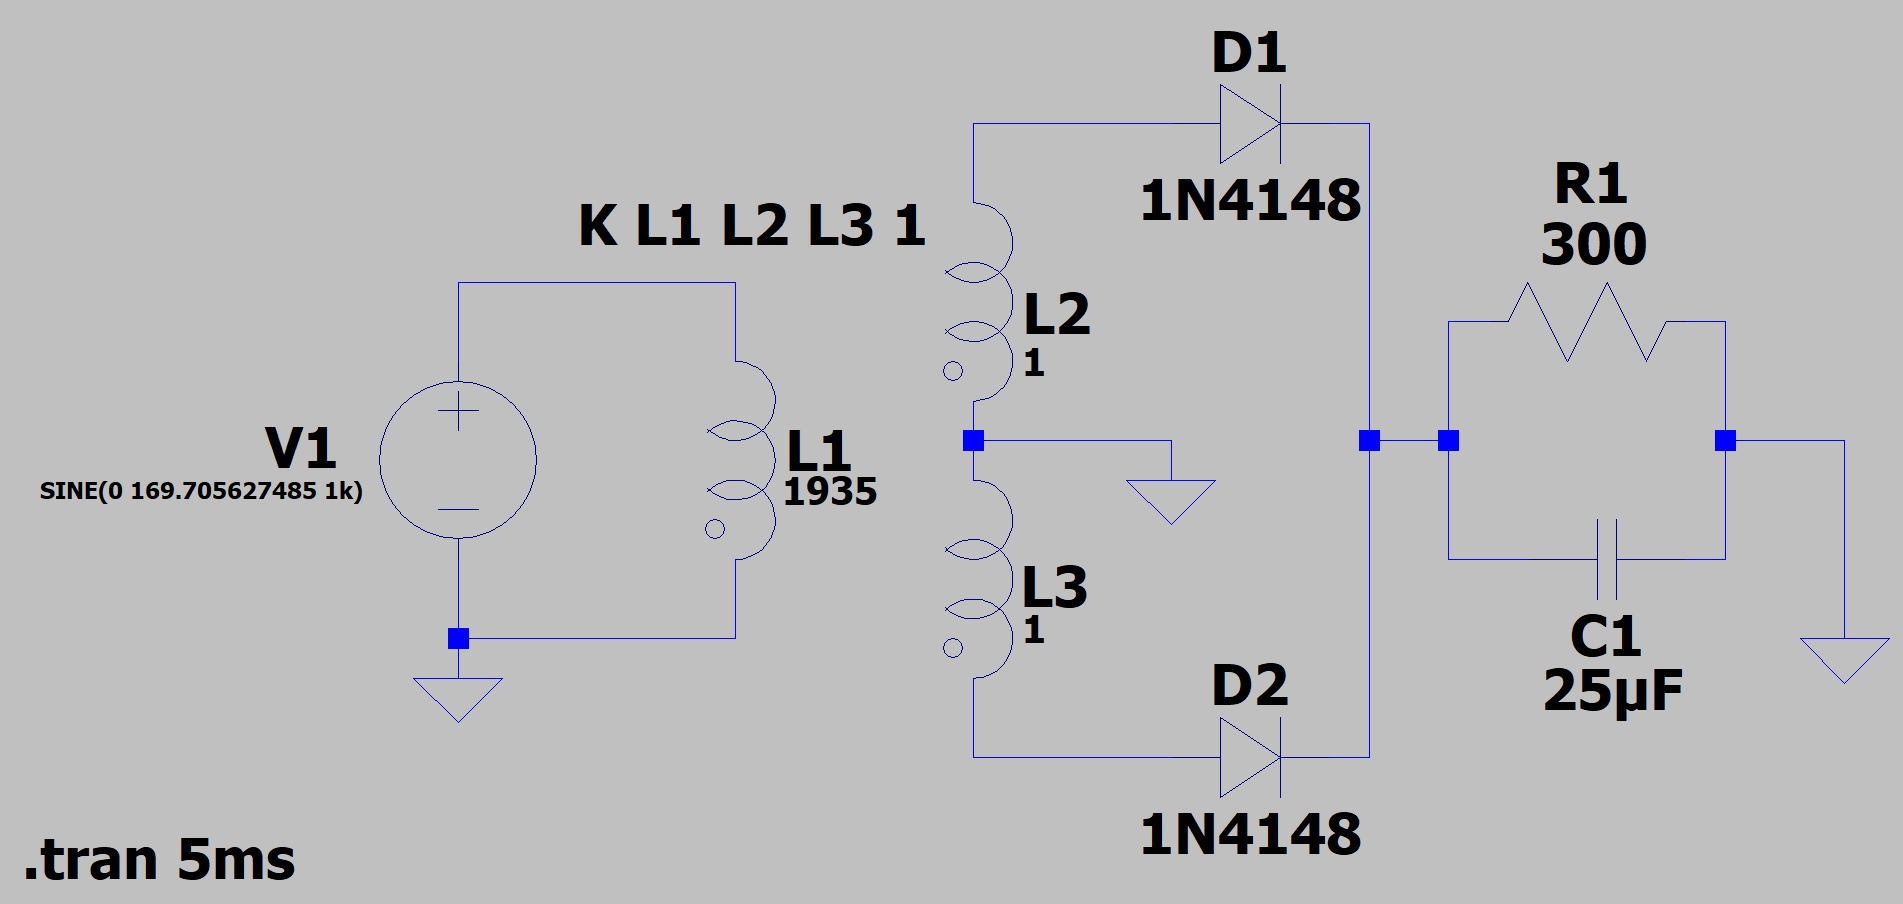
\includegraphics[width=\linewidth]{images/Schematic.png} 
            \caption{Schematic} 
            \vspace{4ex}
        \end{minipage}%%
        ~
        \begin{minipage}[b]{0.5\linewidth}
            \centering
            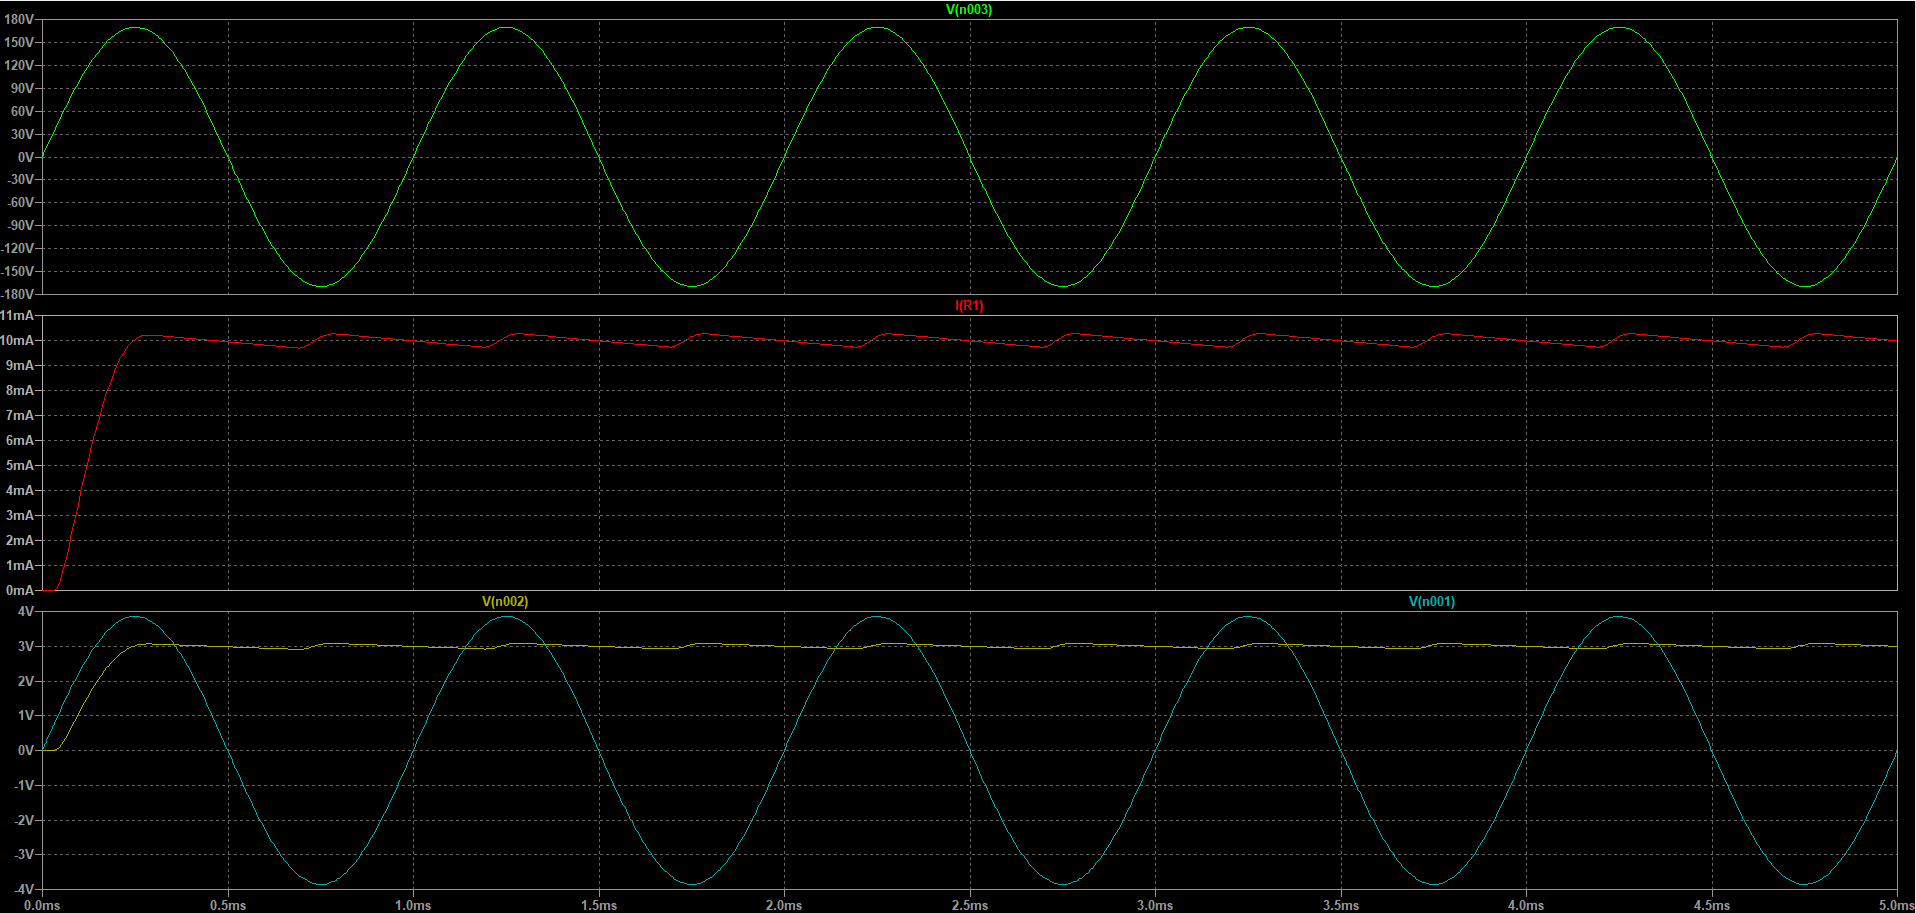
\includegraphics[width=\linewidth]{images/Simulations.png} 
            \caption{Simulations} 
            \vspace{4ex}
        \end{minipage}
        \begin{minipage}[b]{0.5\linewidth}
            \centering
            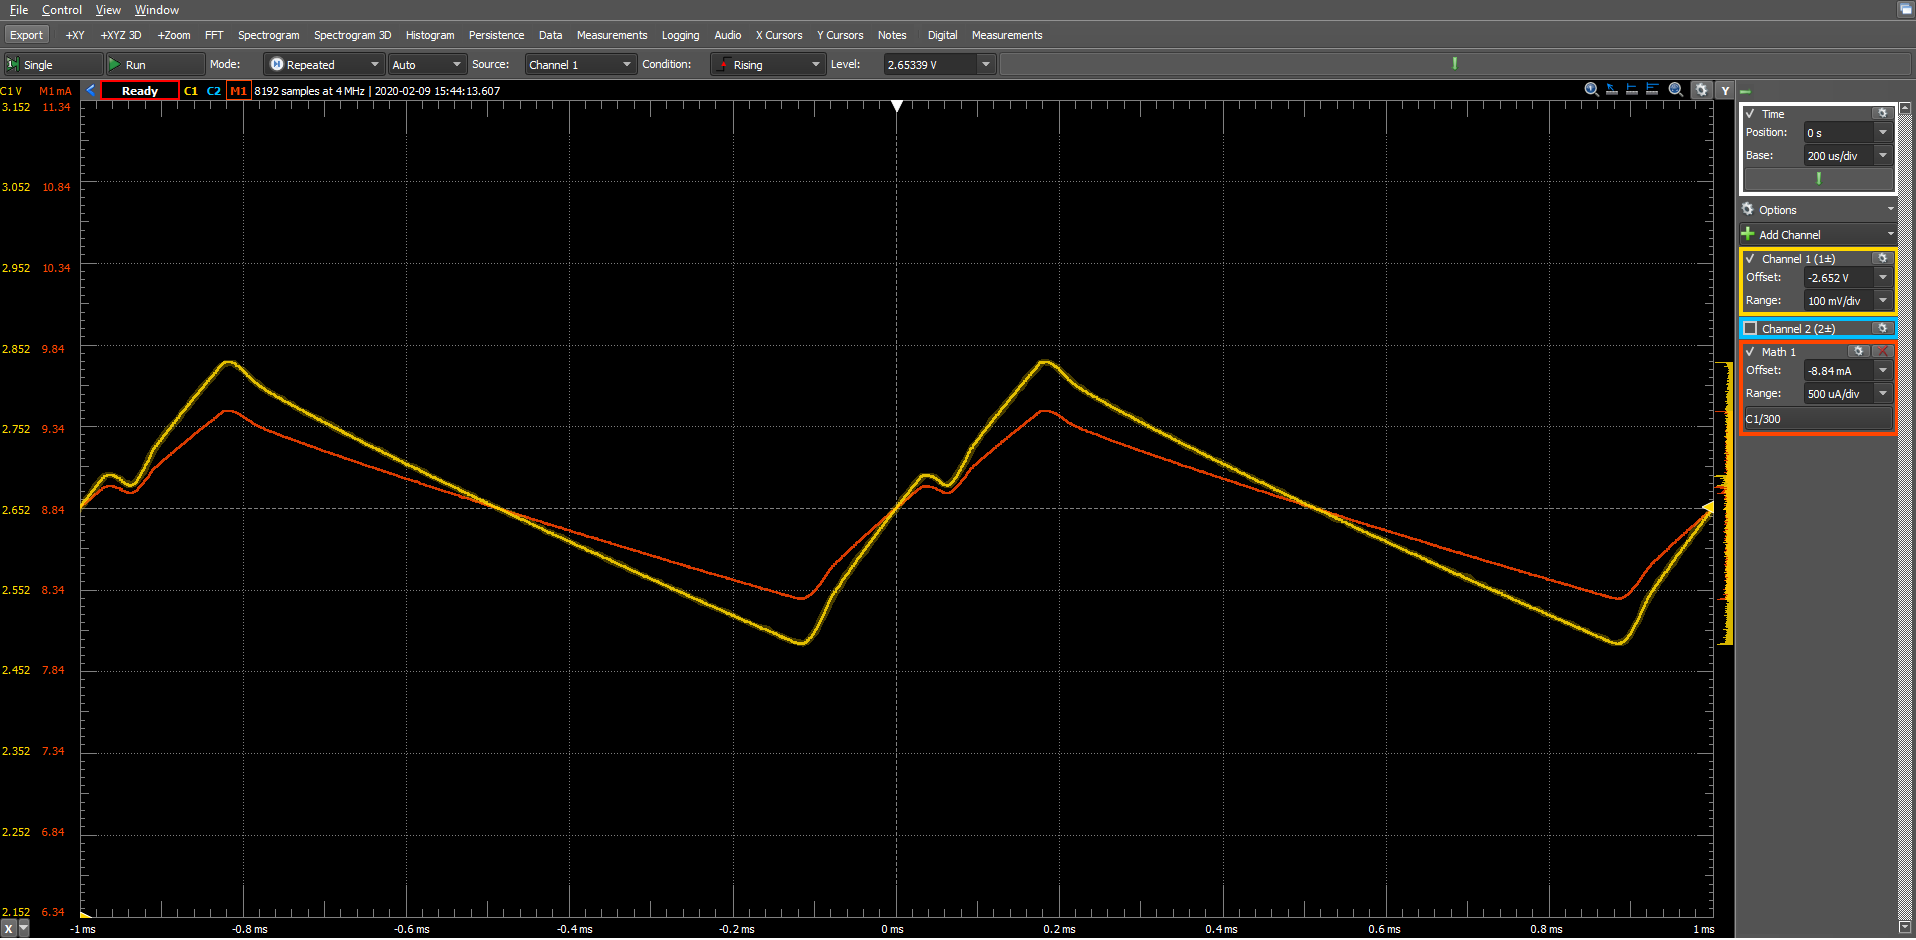
\includegraphics[width=\linewidth]{images/Measurements.png} 
            \caption{Measurements} 
            \vspace{4ex}
        \end{minipage}%%
        \begin{minipage}[b]{0.5\linewidth}
            \centering
            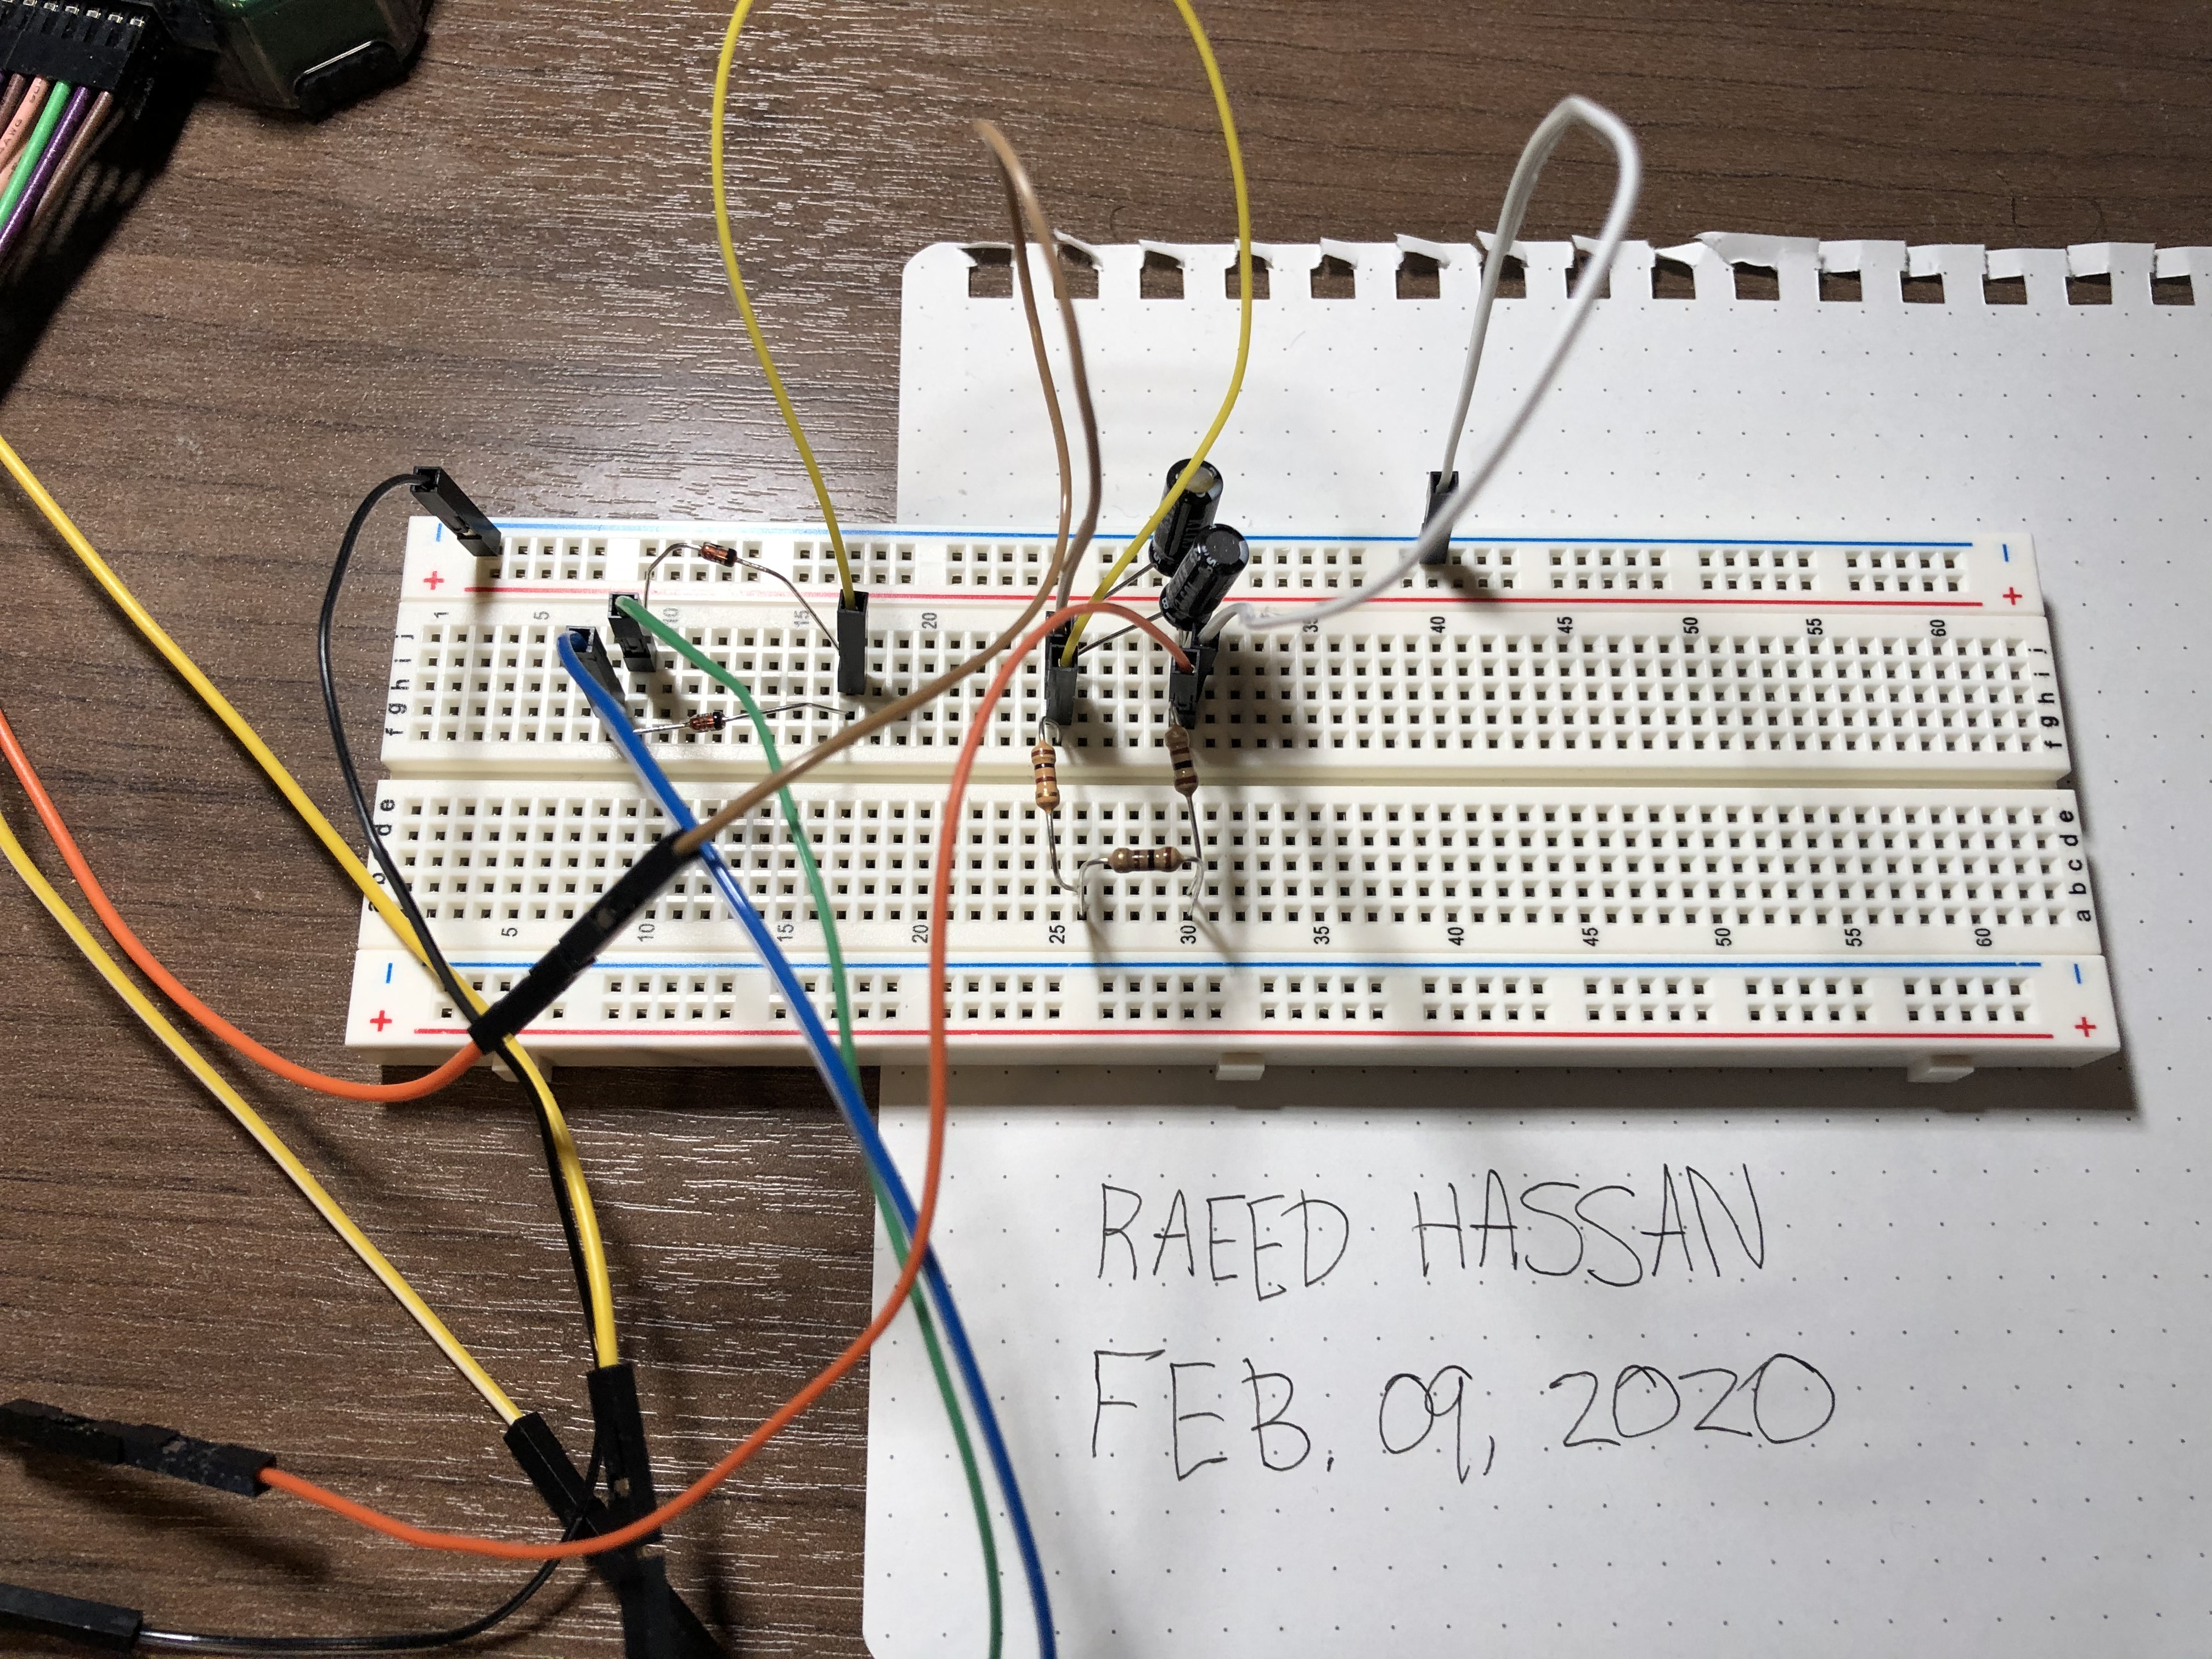
\includegraphics[width=0.74\linewidth]{images/Circuit.png} 
            \caption{Circuit} 
            \vspace{4ex}
        \end{minipage}%%
    \end{figure}
\end{landscape}
\end{document}